% !TeX root = ../main.tex
% Add the above to each chapter to make compiling the PDF easier in some editors.

\chapter{Background and Related Work}\label{chapter:background}
This chapter introduces the technical background and related work for the thesis. It establishes the foundation for the thesis by introducing the concepts of blockchain, smart contracts and specifically smart contracts on the Algorand blockchain network. Furthermore, challenges related to smart contract security and testing are explored, underlining the importance of fuzzing as a relatively novel testing tool in the space. Existing projects in the field of smart contract fuzzing are examined, with the focus on deriving evaluation methods for our own fuzzer.

\section{Blockchain}
Bitcoin was first introduced in 2008 by an anonymous person or group of people under the name of Satoshi Nakamoto \cite{nakamoto_bitcoin_2008}. The purpose of the project was to facilitate online payments without them having to go through a financial institution. Previous solutions were hindered by the double-spend problem, where a user can counterfeit the currency if there isn't a trusted central authority keeping track of the different transactions and the balances. Bitcoin solved this problem with a peer-to-peer network. In this network the nodes keep track of all the transactions that have been committed in a public ledger. These transactions are added to into block which are then chained together through cryptographic hashes. The nodes in the network keep track of the longest chain of blocks and accept the longest chain as the valid one. This is called the \ac{PoW} consensus mechanism. These nodes are incentivized to keep the network secure by receiving a reward in the form of newly minted bitcoins for every block they add to the chain. This process is called \textit{mining}. The \ac{PoW} consensus is computationally expensive, which makes it difficult for an attacker to create a longer chain than the honest nodes. The attacker would have to have more computational power than the rest of the network combined.
This is known as the 51\% attack. The Bitcoin network has been running for over 10 years and has never been compromised.
There are several limitations to this network, such as low transaction throughput and high energy consumption of the \ac{PoW} consensus mechanism.
These limitations have led to the development of new blockchain networks with different consensus mechanisms.

Another interesting feature of Bitcoin that does not have much notoriety is Bitcoin Script. Bitcoin Script is a simple stack-based programming language that is used to define the conditions under which a transaction can be spent. The execution of the script is successful if the stack is empty and failed otherwise. The Bitcoin Script is not Turing-complete, which means that it cannot be used to implement arbitrary programs. Bitcoin Script was not intended to be used for more complex scripts, but it did inspire the creation of new networks that would allow for more complex scripts, later called smart contracts.

\section{Smart Contracts}
The term "Smart Contract" was first coined by Szabo in 1996, to refer to promises between parties and the protocols to perform on these promises stored in digital form \cite{szabo_smart_1996}. This concept was then first connected with blockchain through Ethereum which was proposed by Buterin in 2014 \cite{buterin_ethereum_2014}. Similar to Bitcoin, at the time of its conception Ethereum was also running on a \ac{PoW} consensus, and it had its own currency named Ether. Ethereum went on to expand on the concept of Bitcoin Scripts by allowing arbitrary Turing-complete code to be run on its network. This allowed for the creation of more complex smart contracts, similar to what Szabo had described earlier.
Since the Ethereum network is completely permissionless (meaning anyone can participate without explicit permission from an authority), the addition of smart contracts transformed this network into a "world computer".

The model of the Ethereum smart contracts is pretty simple and since Ethereum was the first blockchain network that supported smart contracts many succeeding networks are more or less similar. For this reason, it is interesting to mention how Ethereum smart contracts work and later to mention how Algorand Smart Contracts differ. Each smart contract has its state (the data of the contract), functions (the code of the contract) and an Ethereum account connected to this contract. The state of the contract is stored in the Ethereum blockchain and is accessible to anyone. The account of the contract is not controlled by a user but only by the code of the corresponding contract. The functions of the contract are the code that is executed when the contract is called. These functions have access not only to the state of the contract, but also to the state of the blockchain. This means that the functions can read the state of other contracts and even call their functions. Also, the function has access to the address of the caller and the amount of ether that the caller may have sent. When a function is called, it is executed by all the nodes in the network. This means that the function is executed in a deterministic way and the result is the same for all the nodes. Because of this, the execution of the function can be expensive for the nodes. Therefore, the caller of the function has to pay a fee for the execution. This fee is calculated based on the amount of computational resources that the function consumes. This means that the more complex the function is, the more expensive it is to execute. The fee is paid in ether and is collected by the nodes that execute the function as an incentive. The fee is also used to prevent denial-of-service attacks, where a malicious user would try to execute a function that consumes a lot of resources and thus make the network unusable.

Allowing anyone to deploy and run arbitrary code on the network has led to the creation of a large ecosystem of \acp{dApp} \cite{wu_empirical_2019}. These \acp{dApp} are similar to traditional web applications, but they are not controlled by a single entity. Instead, they are controlled by the code that is deployed on the network. Also, once deployed the code of these smart contracts cannot be changed due to the immutability property of the blockchain. This is a double-edged sword, as it means that no code fixes can be applied if there is a bug or a security vulnerability. Usually smart contracts control large sums of digital currencies or digital assets, which makes them a very attractive target for attackers. For these two reasons combined, it is of utmost importance to ensure the security of the smart contract before they are deployed.


\section{Smart Contract Security} \label{section:smart_contract_security}
As we already laid out the importance of smart contract security, we will now explore the different types of vulnerabilities that can be found in smart contracts.
Keeping smart contracts secure is compromised of two parts: writing vulnerability free smart contract code and also ensuring that off-chain operations (such as managing an administrating account) are conducted safely. We will be focusing on the first part.

Smart contracts have a lot of idiosyncrasies that set them apart from usual computer programs. Therefore, the types of vulnerabilities that we face when developing smart contracts are usually specific to the world of blockchain and they often differ from one blockchain network to the other. The following list is a non-exhaustive list of vulnerabilities that can be found in smart contracts \cite{he_smart_2020}:
\begin{itemize}
    \item \textbf{Reentrancy} - One of the most iconic vulnerabilities, which has lead to the loss of millions of dollars in cryptocurrencies \cite{pcaversaccio_chronological_nodate}. Functions in Ethereum are not executed atomically. This means that the execution of a function can be interrupted by another function call. This can lead to a vulnerability where a malicious user can call the same function multiple times before the first execution is finished. In this manner, the malicious user could be able to drain the funds of the contract.
    \item \textbf{Integer Overflow and Underflow} - This vulnerability is not specific to smart contracts, but it is prevalent in smart contracts due to the fact that most networks use fixed-size integers. This means that the maximum value of an integer is usually 2\textsuperscript{256}-1. If the result of an operation on integers is larger than the maximum value, the result will overflow and the integer will wrap around to 0. This can lead to a vulnerability where a malicious user can overflow the balance of the contract and drain all the funds.
    \item \textbf{Timestamp Dependence} - The execution environment of the smart contract is managed by the miner of the block. If some logic of the contract depends on the timestamp variable, the miner can manipulate this variable to his advantage.
    \item \textbf{Front-running} - Every transaction on blockchain networks first becomes visible in the mempool prior to being executed. This visibility enables those on the network to view and act on a transaction before it is added to a block. Such exposure can be exploited by malicious actors to manipulate how a transaction is carried out.
    \item \textbf{Resource Limit Vulnerabilities} - As already mentioned above the execution of a function in most blockchain will incur a cost on the caller. If a function is too complex, the costs of executing it might exceed certain limitations of the network or the funds of the contract. This can lead to certain functions of the contract being unusable after a while. An example of this would be calling a function that pays out funds to users from a large array. If the users in the array are too many, the function might not be able to pay out all the users due to the cost of the function exceeding the funds of the contract.
    \item \textbf{Simple Logical Errors} - Although most smart contract are thoroughly scrutinized by the community, still a significant number of vulnerabilities are caused by simple logical errors. These errors cannot be avoided by adding features to your blockchain, as they are inherent in all computer programs written by humans.
\end{itemize}

To deal with these vulnerabilities different tools have been proposed such as static analysis tools, symbolic execution tools and fuzzers, which we will discuss more of on section \ref{section:fuzzing}.

In the next section we will explore the Algorand blockchain network, its smart contracts, how it handles the previously mentioned vulnerabilities and which vulnerabilities are specific to it.

\section{Algorand} \label{section:algorand}
Algorand was initially proposed in 2017 by Chen et al. \cite{chen_algorand_2017}. It sought to improve on previous networks by solving the scalability trilemma, which states that a blockchain network can only have two of the following three properties: security, scalability and decentralization. This is due to the fact that previous networks relied on a consensus mechanism that was computationally expensive and thus limited the transaction throughput of the network. Algorand solved this problem by introducing a new consensus mechanism called \ac{PPoS}. This consensus mechanism has the advantage of being computationally inexpensive and thus allows the network to scale. The network is permissionless, which means that anyone can participate in the consensus. The consensus mechanism is also Byzantine fault tolerant. The network can still function even if up to 1/3 of the nodes in the network are malicious. According to the authors, the possibility of a fork in the network is 10\textsuperscript{-18}, meaning the network practically achieves instant finality of a transaction, from the moment it enters the ledger. This is different from Bitcoin where the finality of a transaction is probabilistic and it increases as more blocks are added to the chain. For Bitcoin finality is usually considered reached after 6 confirmations (meaning 6 blocks after the one containing the interesting transaction). At the time of this writing, new blocks are produced at an average of 3.5 seconds and can hold up to 25000 transactions, which results in a transaction throughput of 7150 \ac{TPS} \cite{noauthor_algorand_nodate-3}.

The native currency of the Algorand network is called Algo, and it has a maximum supply of 10 Billion Algos. The smallest unit of Algo is called a microAlgo and it is equal to 0.000001 Algo. The Algo is used to pay the transaction fees of the network and also to participate in the consensus. Different from the Ethereum gas fee, Algorand fees are only paid if the transaction is included in a block. Transaction fees are calculated based on congestion of the network, but because of the high TPS most transactions can use the minimum base fee of 0.001 Algos. In addition to the fees, Algorand has also \ac{MBR} for its accounts. The \ac{MBR} acts as a deposit to rent space on the blockchain. Every time the amount of stored data on the blockchain increases, the \ac{MBR} of the associated account also increases. When the space is liberated by deleting data, the \ac{MBR} is also decreased. All accounts have a base \ac{MBR} of 0.1 Algo.

One of the most interesting features of the Algorand network is the ability to perform an \texttt{Atomic Transfer} \cite{noauthor_atomic_nodate}. This way, up to 16 transactions are grouped in a transfer where they all succeed or fail together. This is useful in cases where a user wants to perform multiple transactions that are dependent on each other. Atomic transfers can also be used to allow complete strangers to trade. All the required transactions can be added into an atomic transfer and then be independently signed by all the participants. When all the participants have signed the transfer, it can be submitted to the network and all the transactions will be executed. This feature is also relevant to the way Algorand handles payments to smart contracts.

A powerful feature of the protocol is the ability to rekey an account. What this means is being able to change the authoritative spending private key of an account. This is really useful in cases where the user wants to maintain a static public address but wants his private key rotated for security reasons. Rekeying an account is simply accomplished by issuing a transaction with the \texttt{rekey-to} field set to the public address of the new authoritative account.

Different from other networks, the ability to create fungible and non-fungible tokens is directly built into the protocol \cite{noauthor_algorand_nodate-4}. These tokens are created using \ac{ASA} and a special transaction type is required when creating them. On other blockchains a smart contract is required to represent these tokens. Similarly, in Algorand you could have a smart contract to create and control the tokens, but it is not mandatory.

Smart signatures are another feature of the Algorand network, which should not be confused with smart contracts. They are similar to the Bitcoin Scripts. They contain logic that is used to sign a transaction. This logic is then submitted together with the transaction. The logic is then executed by the nodes in the network and if the execution is successful, the transaction is signed and submitted to the network.

\subsection*{Algorand Smart Contracts} \label{section:algorand-smartcontracts}
On the Algorand network smart contracts are written with the \ac{TEAL}, which is a Turing-complete assembly-like language that is interpreted by the \ac{AVM} \cite{noauthor_introduction_nodate}.
Since \ac{TEAL} is a low-level language, it is difficult for developers to write smart contracts directly in it.
For this reason, different high-level solutions that compile to \ac{TEAL} have been developed, such as Reach \cite{noauthor_reach_nodate}, PyTeal \cite{noauthor_pyteal_nodate}, Beaker \cite{noauthor_beaker_nodate} and TEALScript \cite{noauthor_algorandfoundationtealscript_nodate}.
The \ac{TEAL} contracts can be deployed and remotely called from any node in the Algorand blockchain. An on-chain instantiation of an Algorand smart contract is called an \textit{Application}. Special transactions, named \textit{Application Call transactions}, are required to trigger the different functions of the application. Similar to Ethereum smart contracts, an application can modify state, access on-chain values and execute transactions. Each application has an associated account, that only the application can control.

An application can store state in three different ways \cite{noauthor_contract_nodate}:
\begin{itemize}
    \item \textbf{Global Storage} - This is stored on the application itself and only the application can modify it. It allows for the storage of up to 64 key-value pairs. The amount of required storage must be determined on creation and it cannot be changed afterwards.
    \item \textbf{Local Storage} - Similarly to global storage, it is also determined on creation and cannot be change. The maximum amount of key-value pairs is 16. The difference is that local storage is stored on the account that called the application. The local storage of an account is allocated after an account submits an \textit{opt-in} application call. The user can also remove the local storage from his account by submitting a \textit{clear state} application call.
    \item \textbf{Box Storage} - Box storage is similar to global storage, the only meaningful difference being box storage can be dynamically allocated. The box id is required when making an application call for the box storage to be allocated or to be read.
\end{itemize}
Since the state is stored on the blockchain, it is publicly available to anyone. This means it can be read by clients but also by other applications. This allows for the creation of more complex applications that interact with each other.

Smart contracts are implemented with two independent programs: the \textit{Approval Program} and the \textit{Clear State Program}. When making an application call transaction, one can choose form the following transaction types \cite{noauthor_overview_nodate}:
\begin{itemize}
    \item \textbf{NoOp} - Generic application call to execute the Approval Program.
    \item \textbf{OptIn} - Begins participation and enables local storage for an application.
    \item \textbf{DeleteApplication} - Deletes the application and all associated data.
    \item \textbf{UpdateApplication} - Updates the \ac{TEAL} programs for the application. Global and local state requirements cannot be updated and the current state does not change.
    \item \textbf{CloseOut} - Account can end their participation on the contract and clear the local storage. This call can fail and the account can remain opted-in.
    \item \textbf{ClearState} - Similar to CloseOut, but the account will be opted-out regardless if the call succeeds or fails. In other words, the local state of the account associated with this application will be forcefully cleared.
\end{itemize}

Contracts often require data stored within the ledger. To maintain a high level of performance, the \ac{AVM} restricts how much of the ledger can be accessed by an application during execution. This is implemented by having references passed to an application call transaction, which denote the on-chain data the application could access. These references are passed as reference arrays to the call and they may contain the following types of references: Accounts, Assets (\ac{ASA}), Applications and Boxes.

When a smart contract developer want to expose functions (or methods) he can use the \ac{ABI} specification defined in \ac{ARC} 4 \cite{noauthor_arcsarcsarc-0004md_nodate}. This way clients can easily interact with the application. Adhering to the \ac{ABI} specification is not mandatory and many contracts are written without it. Method parameters can have the following types:
\begin{description}
    \item[uintN] An N-bit unsigned integer, where 8 <= N <= 512 and N \% 8 = 0
    \item[byte]	An alias for uint8
    \item[bool]	A boolean value that is restricted to either 0 or 1. When encoded, up to 8 consecutive bool values will be packed into a single byte
    \item[ufixedNxM] An N-bit unsigned fixed-point decimal number with precision M, where 8 <= N <= 512, N \% 8 = 0, and 0 < M <= 160, which denotes a value v as v / (10\^M)

        \item[{type[N]}] A fixed-length array of length N, where N >= 0. type can be any other type
    \item[address] Used to represent a 32-byte Algorand address. This is equivalent to byte[32]

        \item[{type[]}] A variable-length array. type can be any other type
    \item[string] A variable-length byte array (byte[]) assumed to contain UTF-8 encoded content
        (T1,T2,...,TN) A tuple of the types T1, T2, …, TN, N >= 0
    \item[reference] A uint8 parameter that points to an account, asset or application in the references array.
    \item[transaction] A parameter that points to a transaction in a \textit{transaction group}.
\end{description}

In contrast to Ethereum, application calls on Algorand are not marked as payable or asset transfer etc. To send a payment or an asset transfer with an application call Algorand makes use of its atomic transfers feature. When a client sees that a payment is need for a method then he would need to add the payment and the application call in an atomic transfer. This way the payment and the application call will be executed together and the payment can be evaluated by the contract. These transactions can also be noted in the \ac{ABI} as \texttt{pay} for payments, \texttt{acfg} for asset config/create, \texttt{axfer} for asset transfer, \texttt{afrz} for asset freeze and \texttt{keyreg} for key registration.


\subsection*{Algorand Smart Contract Security} \label{section:algorand-smartcontracts-security}
Smart contracts on Algorand have their own set of common vulnerabilities. Most of the previously mentioned vulnerabilities (section \ref{section:smart_contract_security}) are not applicable to Algorand smart contracts for the following reasons:
\begin{itemize}
    \item \textbf{Reentrancy} - Application calls and payment/asset transfers are different types of transactions in Algorand. Payment and asset transfers do not trigger any code execution. Also, an application cannot make a call to itself directly or indirectly. This means that reentrancy is not possible.
    \item \textbf{Integer Overflow and Underflow} - All overflows and underflows halt the execution and fail the current transaction.
    \item \textbf{Front-running} - The block proposer in Algorand is chosen randomly. The proposer cannot know beforehand whether he will be the next proposer. Therefore, the ability to front run is massively mitigated.
    \item \textbf{Time Dependence} - Although Algorand smart contracts can use a timestamp variable, it is very difficult to manipulate it. Similar to front-running, the block proposer cannot know beforehand whether he will be the next proposer.
\end{itemize}

From the previous list of vulnerabilities, only \textbf{Resource Limit Vulnerabilities} and \textbf{Simple Logical Errors} are applicable to Algorand smart contracts. The following list is a non-exhaustive list of Algorand specific vulnerabilities that are commonly encountered \cite{crytic_building-secure-contractsnot-so-smart-contractsalgorand_nodate,sun_panda_2023}:
\begin{itemize}
    \item \textbf{Rekeying} - The \texttt{rekey-to} field is not checked by the smart contract. An attacker could use this to take control of the account associated with the smart contract.
    \item \textbf{Unchecked Group Size} - An attacker can create correct transactions at the particular indices. Then, he can populate the rest of the indices with malicious transactions. When the group size is not checked, the malicious transactions will be executed together with the correct transactions.
    \item \textbf{Uncontrolled update/delete operations} - Update and delete calls can be sent by anyone, and whether the transaction is approved depends on the program logic. Lack of appropriate checks would allow attackers to update the application logic or delete the application.
    \item \textbf{Asset Id Check} - Not checking the asset id, might allow an attacker to transfer assets that are not intended to be transferred.
    \item \textbf{Unchecked receiver} - As we mentioned, a payment or an asset transfer can be grouped together with the application call. The application call and the transfer even though grouped together, have no relation to each other. Developers (for example coming from Ethereum) might assume that the receiver of the transfer is automatically the account of the current application. An attacker could use this to his advantage.
\end{itemize}

These and other similar types of vulnerabilities are present in Algorand smart contracts.
What's common about these vulnerabilities is that they are very simple in nature.
They are not caused by the complexity of the smart contract, but rather by the lack of proper checks.
This simplicity of the common vulnerabilities and how it affected our design choices will be discussed in Chapter \ref{chapter:methodology}.

\section{Fuzzing} \label{section:fuzzing}
The concept of fuzzing can be traced back to the 1980s when Professor Barton Miller at the University of Wisconsin experimented with sending random strings to UNIX utility programs \cite{miller_empirical_1990}.
Out of the programs tested 25\% to 33\% crashed, which at the time was a surprising result.
From this work the first fuzzing tool was built to allow other researchers to conduct similar experiments.

The main idea behind fuzzing is providing random input for the program under test and monitoring its behavior.
The fuzzing process is usually represented by the following steps \cite{manes_art_2019}:
\begin{enumerate}
    \item Input is generated given a fuzzing configuration.
    \item The generated input is evaluated against the program, given a certain bug oracle.
    \item The evaluation results are used to improve the fuzzing configuration.
    \item The process is repeated until the time limit is reached or the bug oracle is satisfied.
\end{enumerate}

\begin{algorithm}
    \caption{Generic fuzzing algorithm}\label{alg:fuzz}
    \begin{algorithmic}
        \item \textbf{Input: } $conf, t_{limit}$
        \item \textbf{Output: } $\mathbb{R} - results$
        \State $\mathbb{R} \gets \emptyset$
        \While{$t_{elapsed} < t_{limit} \land \textbf{Continue}(result)$}
        \State $input \gets \textbf{InputGen}(conf)$
        \State $result, execinfo \gets \textbf{InputEval}(input, O_{bug})$
        \State $conf \gets \textbf{ConfUpdate}(conf, result, execinfo)$
        \State $\mathbb{R} \gets \mathbb{R} \cup \{result\}$
        \EndWhile
    \end{algorithmic}
\end{algorithm}

Because there is a time limit on the fuzzing process, most fuzzers want to prioritize the input that is most likely to trigger a bug.
This is usually done by using different metrics to decide which input is more interesting in this regard.
One of the most popular metrics is code coverage.
The idea is that the input that covers the most code is more likely to trigger a bug.
In such fuzzers, interesting inputs are saved and prioritized based on the rareness of their coverage path.
This measure of how interesting an input is, is often called the \textit{energy} of the input.
To facilitate this, fuzzers usually have an architecture consisting of the following parts \cite{zeller_greybox_2023}:
\begin{itemize}
    \item \textbf{Fuzzer} - Runner of the main fuzzing loop.
    \item \textbf{Schedule} - Defines how the fuzzing should be distributed across the population.
    \item \textbf{Input Generator} - Generates the input for the fuzzing process. There are many different types of input generators, the most popular ones being mutation-based.
    \item \textbf{Seed} - This represents an interesting input that contains that data, the energy and other information about the particular input.
\end{itemize}

\begin{figure}
    \centering
    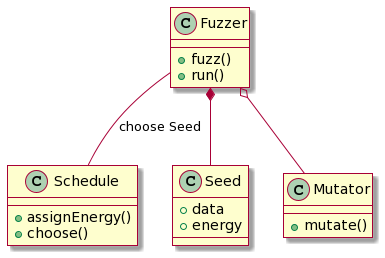
\includegraphics[width=0.8\textwidth]{figures/generic-fuzzer-architecture.png}
    \caption{Generic architecture of a fuzzer}\label{fig:generic-fuzzer-architecture}
\end{figure}

This architecture shown in Figure \ref{fig:generic-fuzzer-architecture} will also be used and extended in our fuzzer.

\section{Related Work}
In this section we will explore the existing work in the field of smart contract fuzzing. Next, we review existing tools that aim to improve the security of Algorand smart contracts. Finally, we present the research gap that our work aims to fill.

\subsection*{Smart Contract Fuzzing}
A number of fuzzers have been developed for smart contracts.
The vast majority of them target Ethereum smart contracts.
Here is a brief overview of the most notable ones:
\begin{itemize}
    \item \textbf{Echidna}: One of the most prominent fuzzers for Ethereum smart contracts is Echidna. Developed by Trail of Bits, Echidna is a property-based fuzzer that tests the contract's invariants using random transactions.
          Echidna has been employed in numerous security audits and has proven to be effective in uncovering bugs in Ethereum contracts \cite{grieco_echidna_2020}.
          It makes use of an EVM implementation written in Haskell called \textit{hevm}, which allows it to run the contracts in a sandboxed environment.

    \item \textbf{ContractFuzzer}: Introduced in 2018, it stands as one of the earliest examples of fuzzing applied to smart contracts \cite{jiang_contractfuzzer_2018}.
          The fuzzer uses static analysis in combination with fuzzing to generate inputs that are more likely to trigger bugs.
          Different from Echidna, it uses a private Ethereum network to run the contracts.
          One big contribution of this work is one of the first introductions of specific bug oracles for ethereum smart contracts.
    \item \textbf{Harvey}: One of the few closed sourced fuzzing engines \cite{wustholz_harvey_2020}.
          It is one of the fuzzers with most industrial use.
          The company Consensys has used it to build their smart contract fuzzing platform called Diligence Fuzzing.
    \item \textbf{Notable non ethereum fuzzers}: There are several other fuzzers like HFContractFuzzer \cite{ding_hfcontractfuzzer_2021}, EOSFuzzer \cite{huang_eosfuzzer_2021}, and AntFuzzer \cite{zhou_antfuzzer_2022}.
          These fuzzers target other smart contract platforms like EOS \cite{noauthor_home_nodate} and Hyperledger Fabric \cite{noauthor_hyperledger_nodate}.

\end{itemize}

\subsection*{Algorand Smart Contract Security}
Algorand, while not as extensively explored as Ethereum in terms of security tooling, has seen efforts directed towards enhancing the security of its smart contracts:
\begin{itemize}
    \item \textbf{Tealer}: This is a static analysis tool that checks for common vulnerabilities in Algorand smart contracts \cite{noauthor_crytictealer_nodate}.
          Most of the checks are based on the vulnerabilities that we mentioned in section \ref{section:algorand-smartcontracts-security}.
          As the vulnerabilities are simple in nature, the tool is capable of detecting most of them.

    \item \textbf{Panda}: It is another static analysis tool for Algorand contracts \cite{sun_panda_2023}.
          Different from Tealer, the user can define custom rules to check for vulnerabilities, aside from the ones that are already implemented.
          The tool has found many vulnerabilities in real world projects which have been acknowledged by the respective teams.
    \item \textbf{AlgoBuilder}: A framework for building \acp{dApp} for Algorand \cite{noauthor_algo_nodate}.
          Included with the framework is a testing tool that allows the developer to write tests for their smart contracts.
\end{itemize}

\subsection*{Research Gap}
Despite the efforts and tools available for ensuring the security of Algorand smart contracts, there exists a significant gap in the domain of fuzzing.
While Ethereum has seen a multitude of fuzzers, Algorand lacks a dedicated fuzzer tailored for its unique smart contract architecture and the \ac{TEAL} scripting language.
In the GitHub repository of Algorand, there is a fuzzer called \textit{TealFuzz}, but the project is currently abandoned, with the last commit being made in 2020 \cite{noauthor_tealfuzz_2023}.

As Algorand continues to gain traction, the complexity of its smart contracts will increase.
The security of these contracts will need to be handled from all angles.
Therefore, a dedicated fuzzer for Algorand smart contracts is a necessary addition to the security tooling of the network.